%% Results
%%=========================================

\chapter{Results}
\label{ch:results}
Below are the results for each test ran in our experiments. These results are analyzed in the next chapter.

%%=========================================

\section{Accuracy on Datasets}
Table \ref{table:accuracy_model_data_sets} contains the accuracy for each model on each of the three datasets of various sizes, as described in section \ref{sec:accuracy_on_datasets}. The accuracy and loss plots for each test are presented below, showing the progression over the epochs.

\begin{table}[H]
    \centering
    \begin{tabular}{|l|l|l|l|}
        \hline 
                                        & \textbf{Small dataset}          & \textbf{Medium dataset}         & \textbf{Big dataset}            \\ \hline
        {\tt VecRep }                   & 16.80\%                         & 25.14\%                         & 55.01\%                         \\ \hline
        {\tt EncDecReg}                 & 41.20\%                         & 55.52\%                         & 95.49\%                         \\ \hline
        {\tt EncDecAtt}                 & \textbf{92.00\%}                & \textbf{97.16\%}                & \textbf{98.75\%}                \\ \hline
    \end{tabular}
    \caption{Test accuracy for each model on each test set, with the best results for each test set highlighted}
    \label{table:accuracy_model_data_sets}
\end{table}

\newpage
\subsection{VecRep}
\subsubsection{Accuracy and Loss}
\resultplots{fig/results/experiment1/small/vecrep/}{plot_accuracy_crop.png}{plot_loss_crop.png}{result1_small_vecrep}{Accuracy and loss for {\tt VecRep} on small dataset}
\resultplots{fig/results/experiment1/medium/vecrep/}{plot_accuracy_crop.png}{plot_loss_crop.png}{result1_medium_vecrep}{Accuracy and loss for {\tt VecRep} on medium dataset}
\resultplots{fig/results/experiment1/big/vecrep/}{plot_accuracy_crop.png}{plot_loss_crop.png}{result1_big_vecrep}{Accuracy and loss for {\tt VecRep} on big dataset}

\newpage
\subsubsection{Confusion Matrix}
\begin{figure}[H]
    \centering
    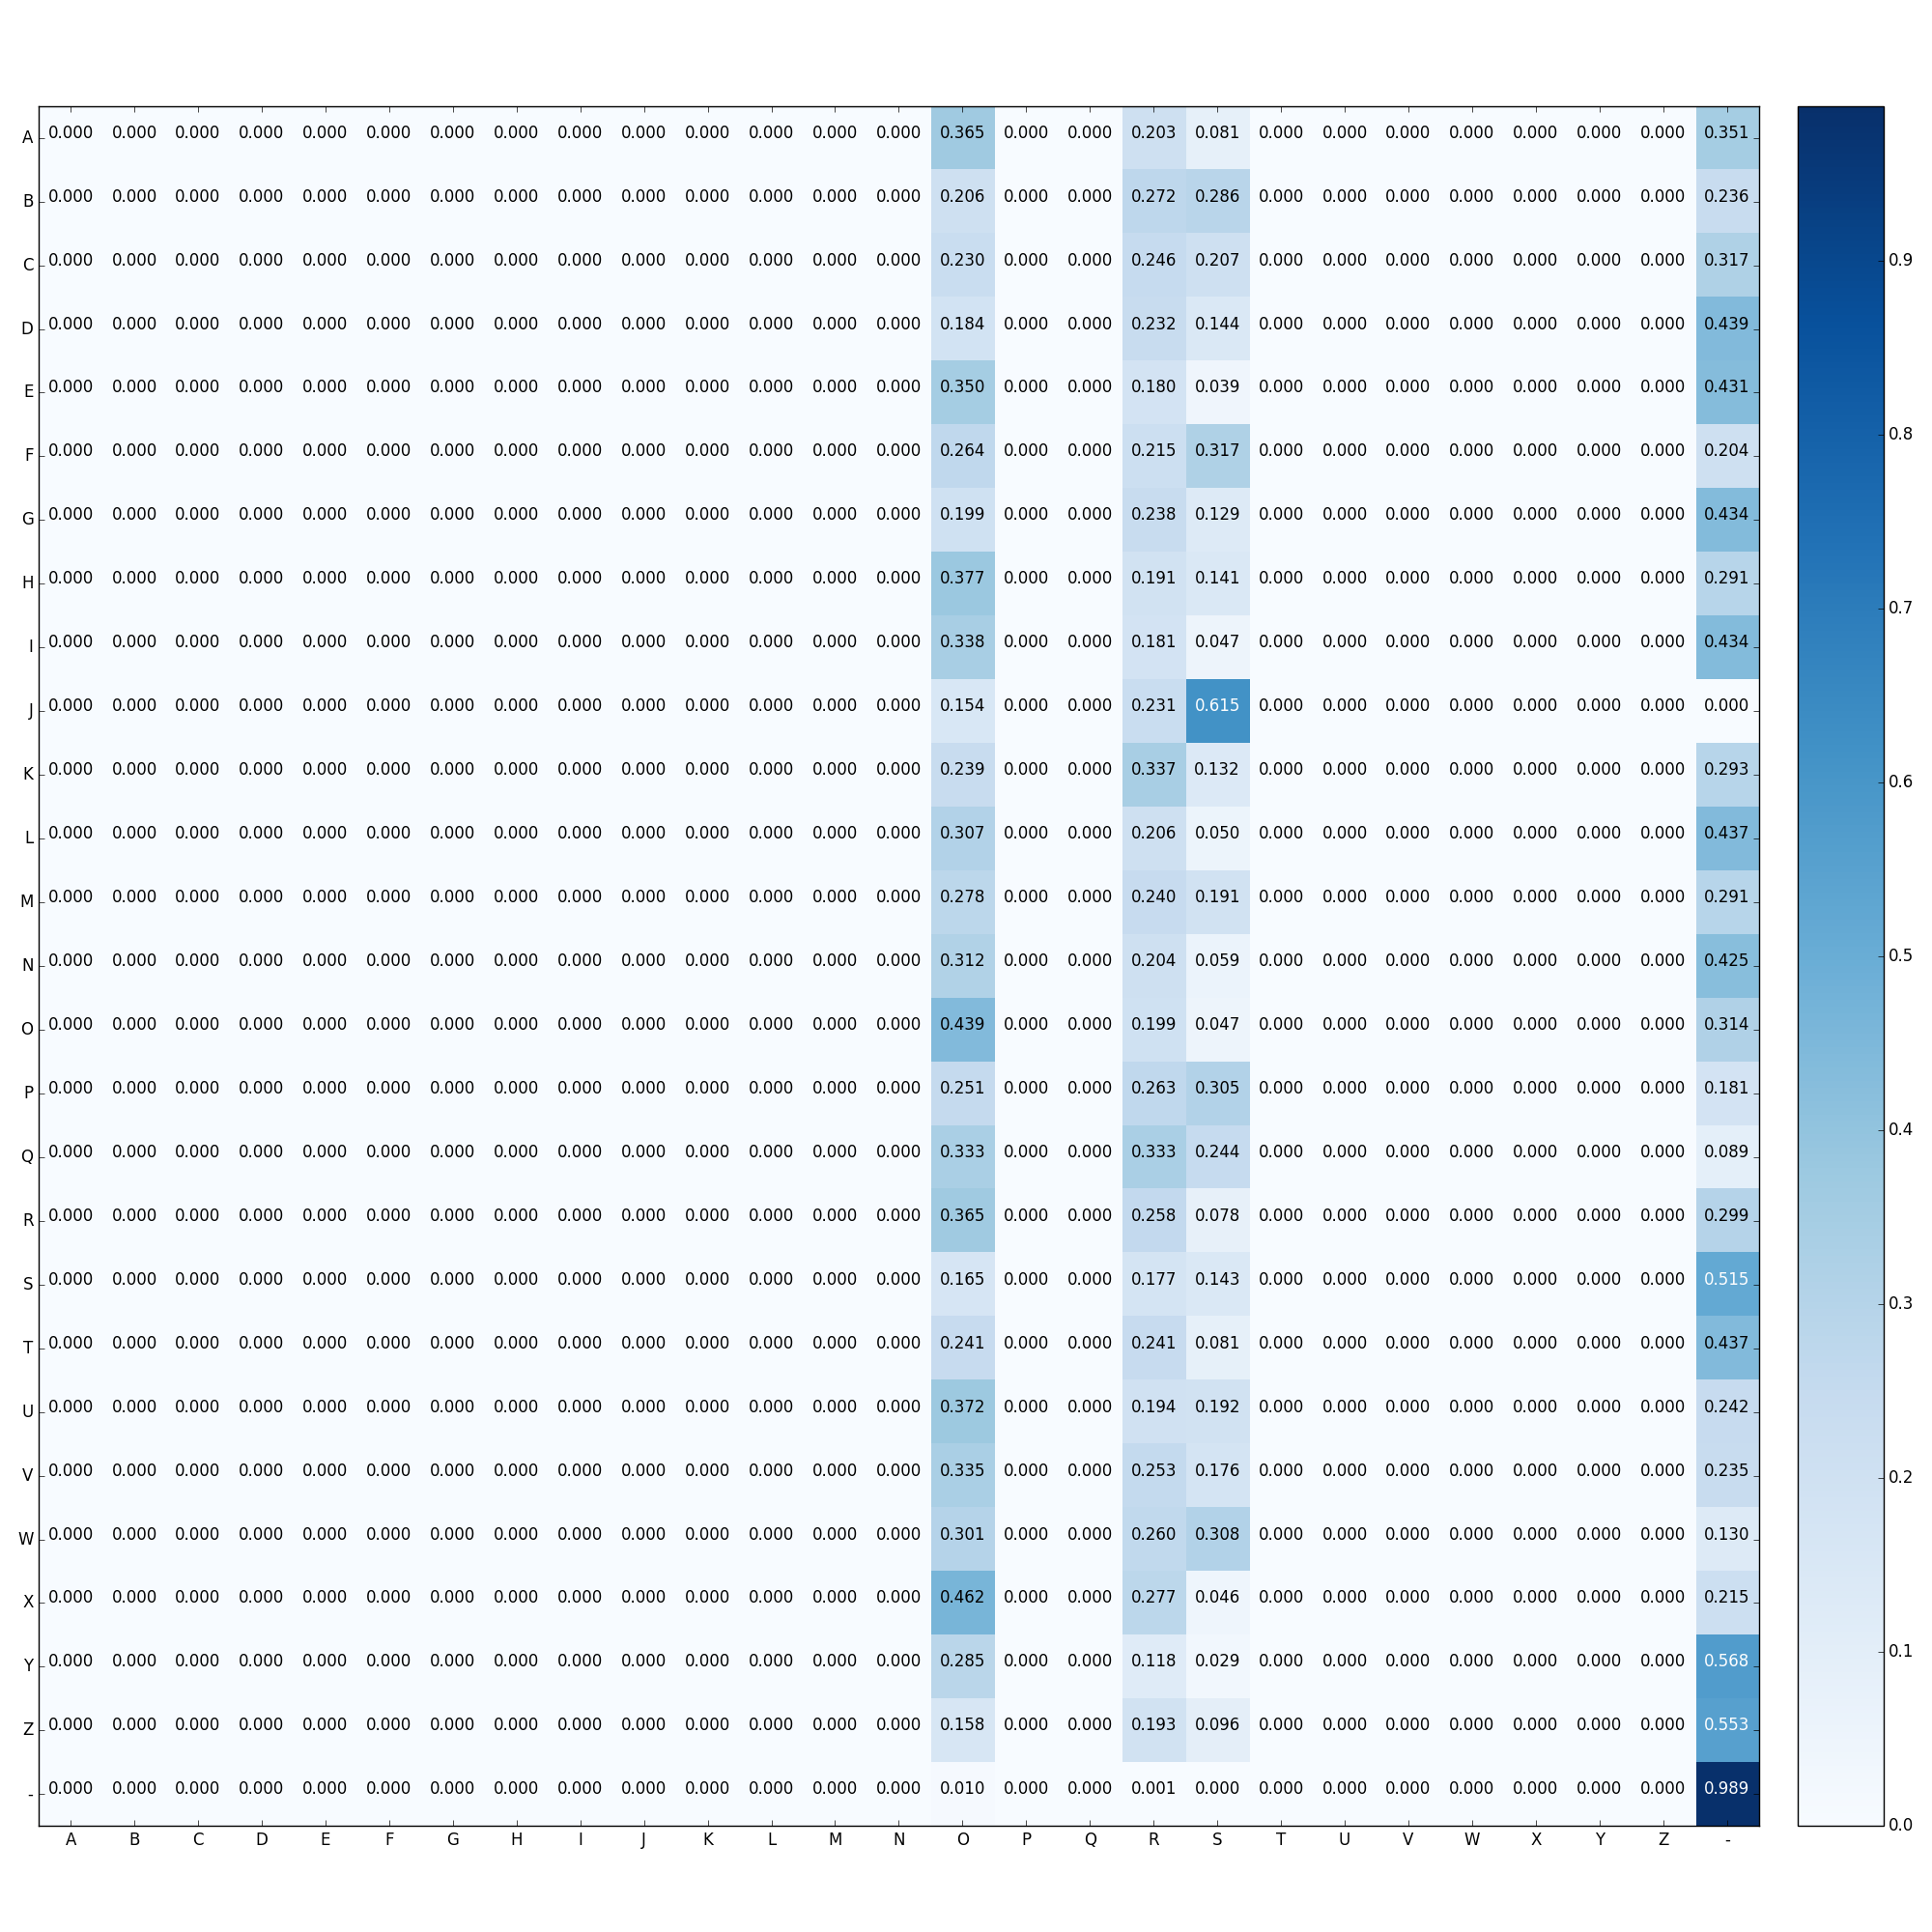
\includegraphics[width=1\textwidth]{fig/results/experiment1/big/vecrep/confusion_matrix.png}
    \caption{Confusion matrix for the best {\tt VecRep} model on the big dataset}
    \label{fig:result1_big_vecrep_confusion_matrix}
\end{figure}

\subsection{EncDecReg}
\subsubsection{Accuracy and Loss}
\resultplots{fig/results/experiment1/small/encdecreg/}{plot_accuracy_crop.png}{plot_loss_crop.png}{result1_small_encdecreg}{Accuracy and loss for {\tt EncDecReg} on small dataset}
\resultplots{fig/results/experiment1/medium/encdecreg/}{plot_accuracy_crop.png}{plot_loss_crop.png}{result1_medium_encdecreg}{Accuracy and loss for {\tt EncDecReg} on medium dataset}
\resultplots{fig/results/experiment1/big/encdecreg/}{plot_accuracy_crop.png}{plot_loss_crop.png}{result1_big_encdecreg}{Accuracy and loss for {\tt EncDecReg} on big dataset}

\newpage
\subsubsection{Confusion Matrix}
\begin{figure}[H]
    \centering
    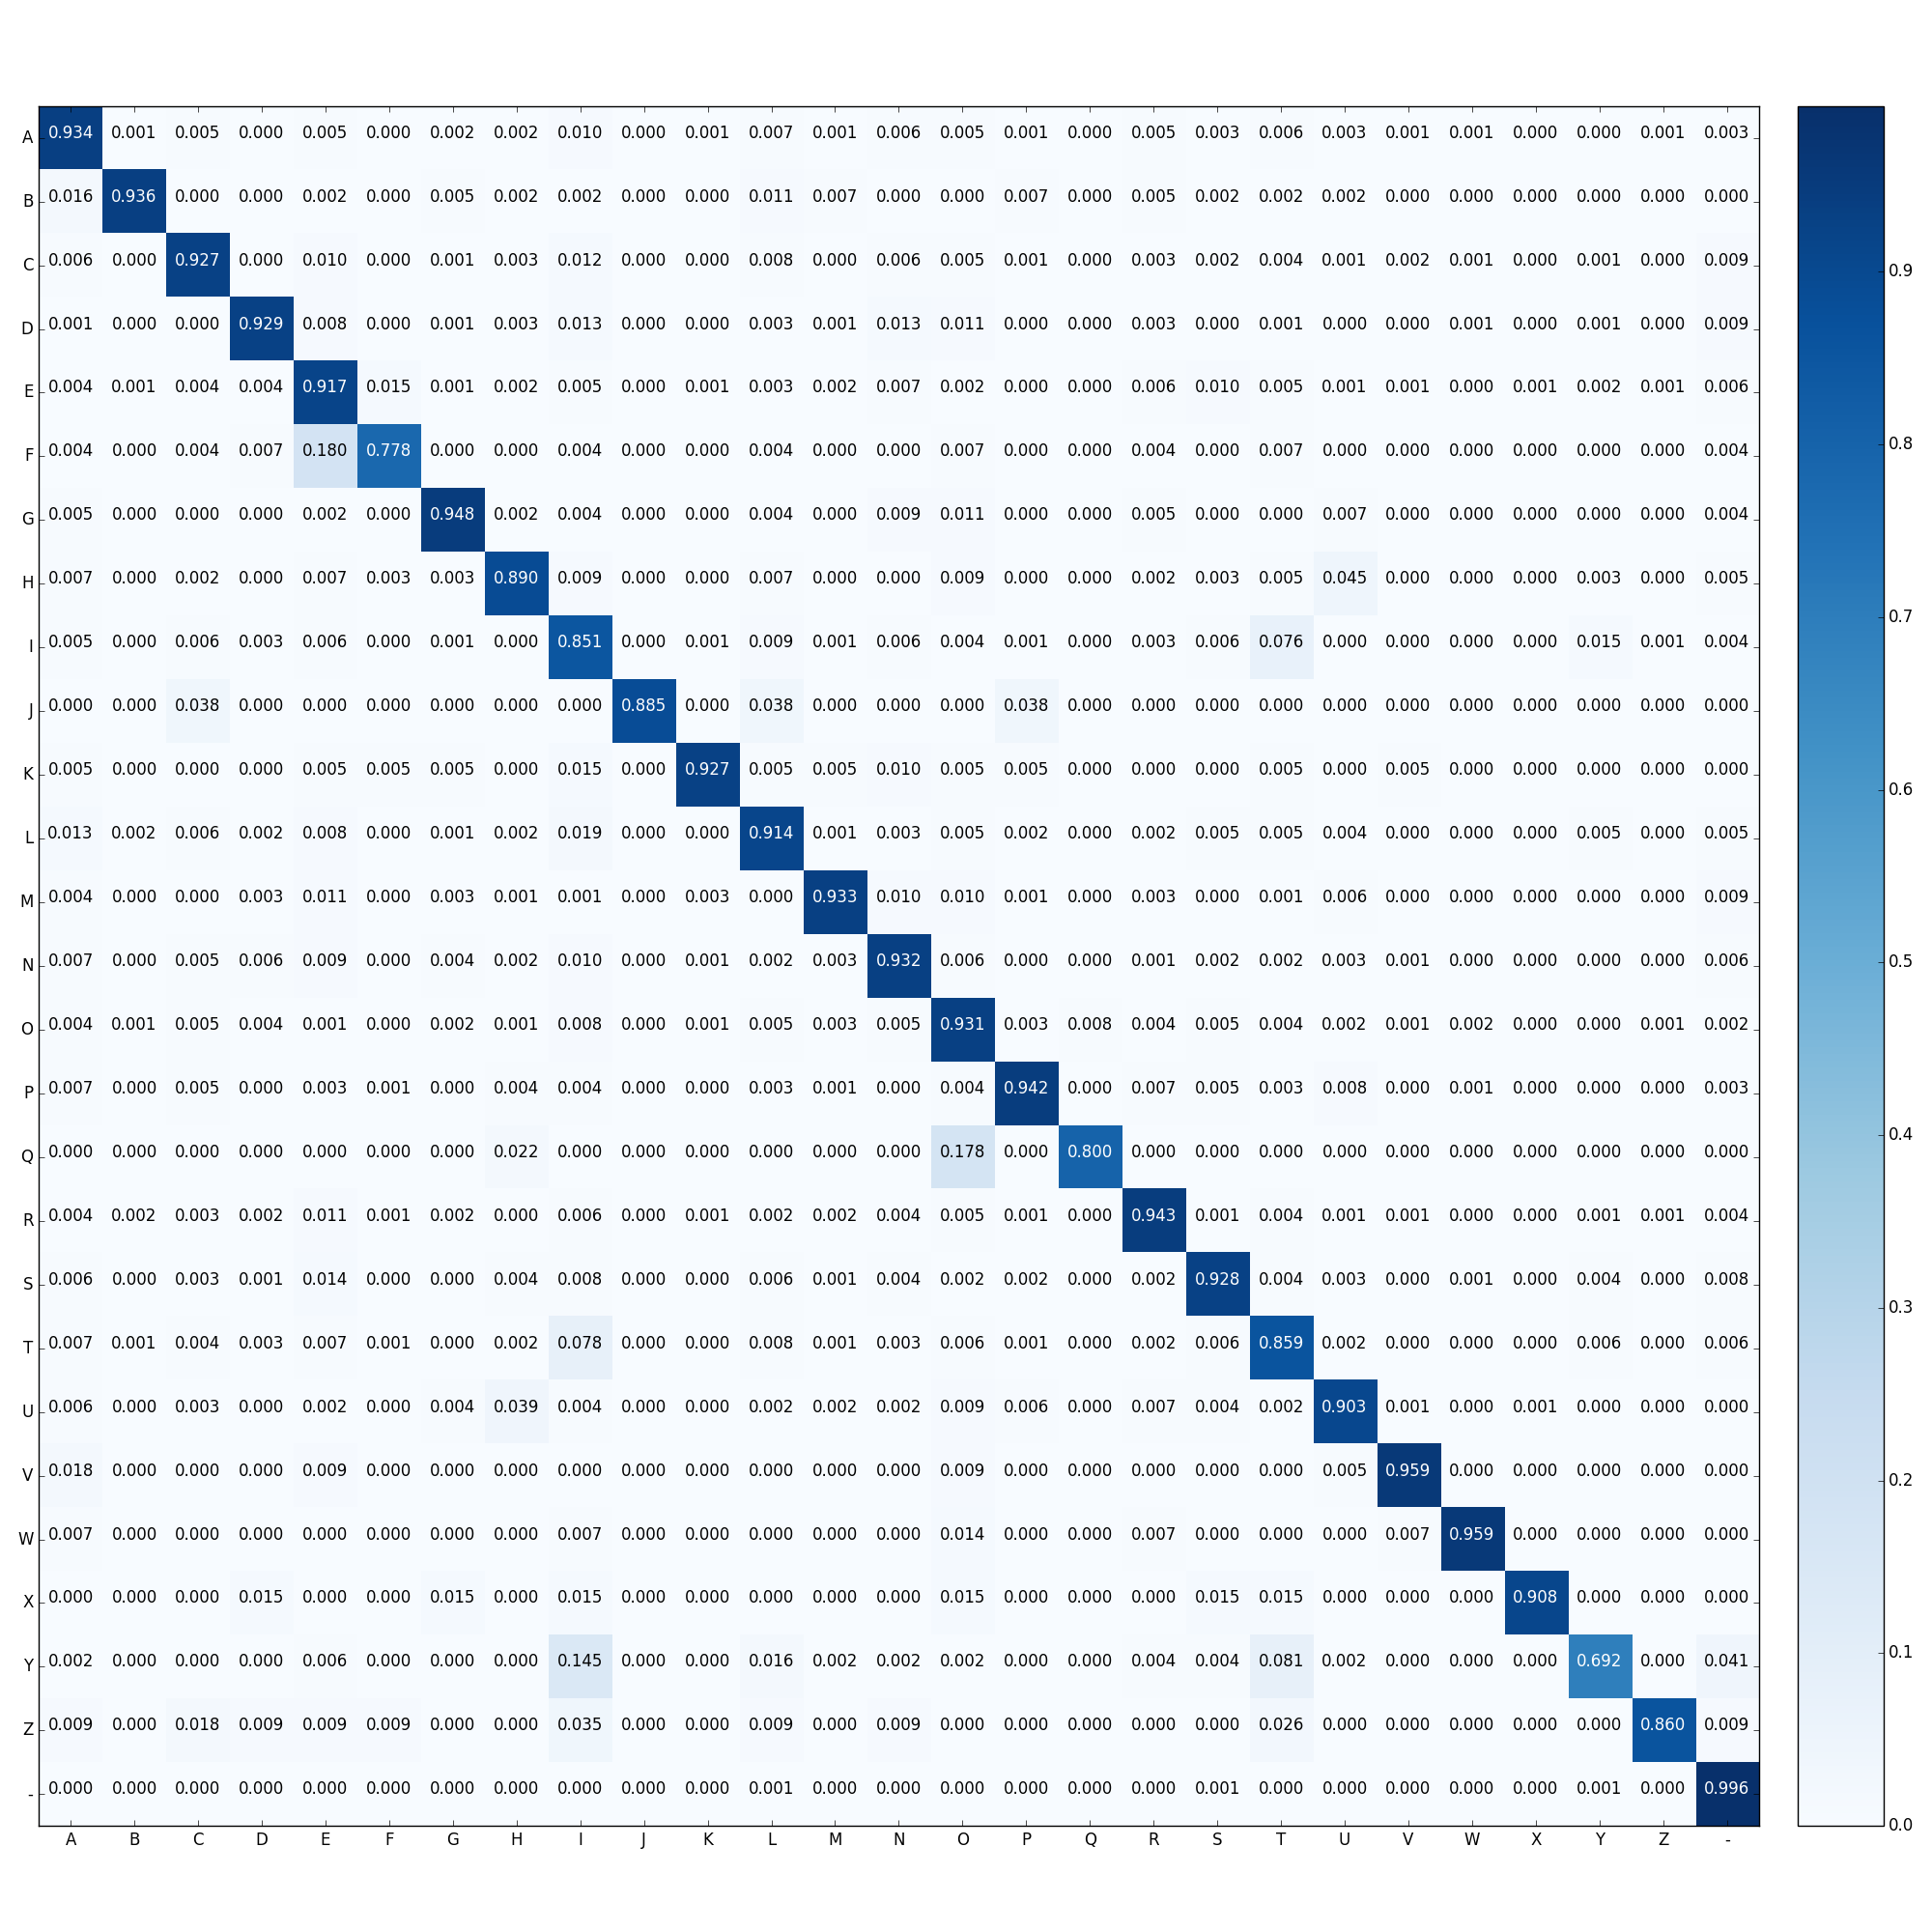
\includegraphics[width=1\textwidth]{fig/results/experiment1/big/encdecreg/confusion_matrix.png}
    \caption{Confusion matrix for the best {\tt EncDecReg} model on the big dataset}
    \label{fig:result1_big_encdecreg_confusion_matrix}
\end{figure}

\subsection{EncDecAtt}
\subsubsection{Accuracy and Loss}
\resultplots{fig/results/experiment1/small/encdecatt/}{plot_accuracy_crop.png}{plot_loss_crop.png}{result1_small_encdecatt}{Accuracy and loss for {\tt EncDecAtt} on small dataset}
\resultplots{fig/results/experiment1/medium/encdecatt/}{plot_accuracy_crop.png}{plot_loss_crop.png}{result1_medium_encdecatt}{Accuracy and loss for {\tt EncDecAtt} on medium dataset}
\resultplots{fig/results/experiment1/big/encdecatt/}{plot_accuracy_crop.png}{plot_loss_crop.png}{result1_big_encdecatt}{Accuracy and loss for {\tt EncDecAtt} on big dataset}

\newpage
\subsubsection{Confusion Matrix}
\begin{figure}[H]
    \centering
    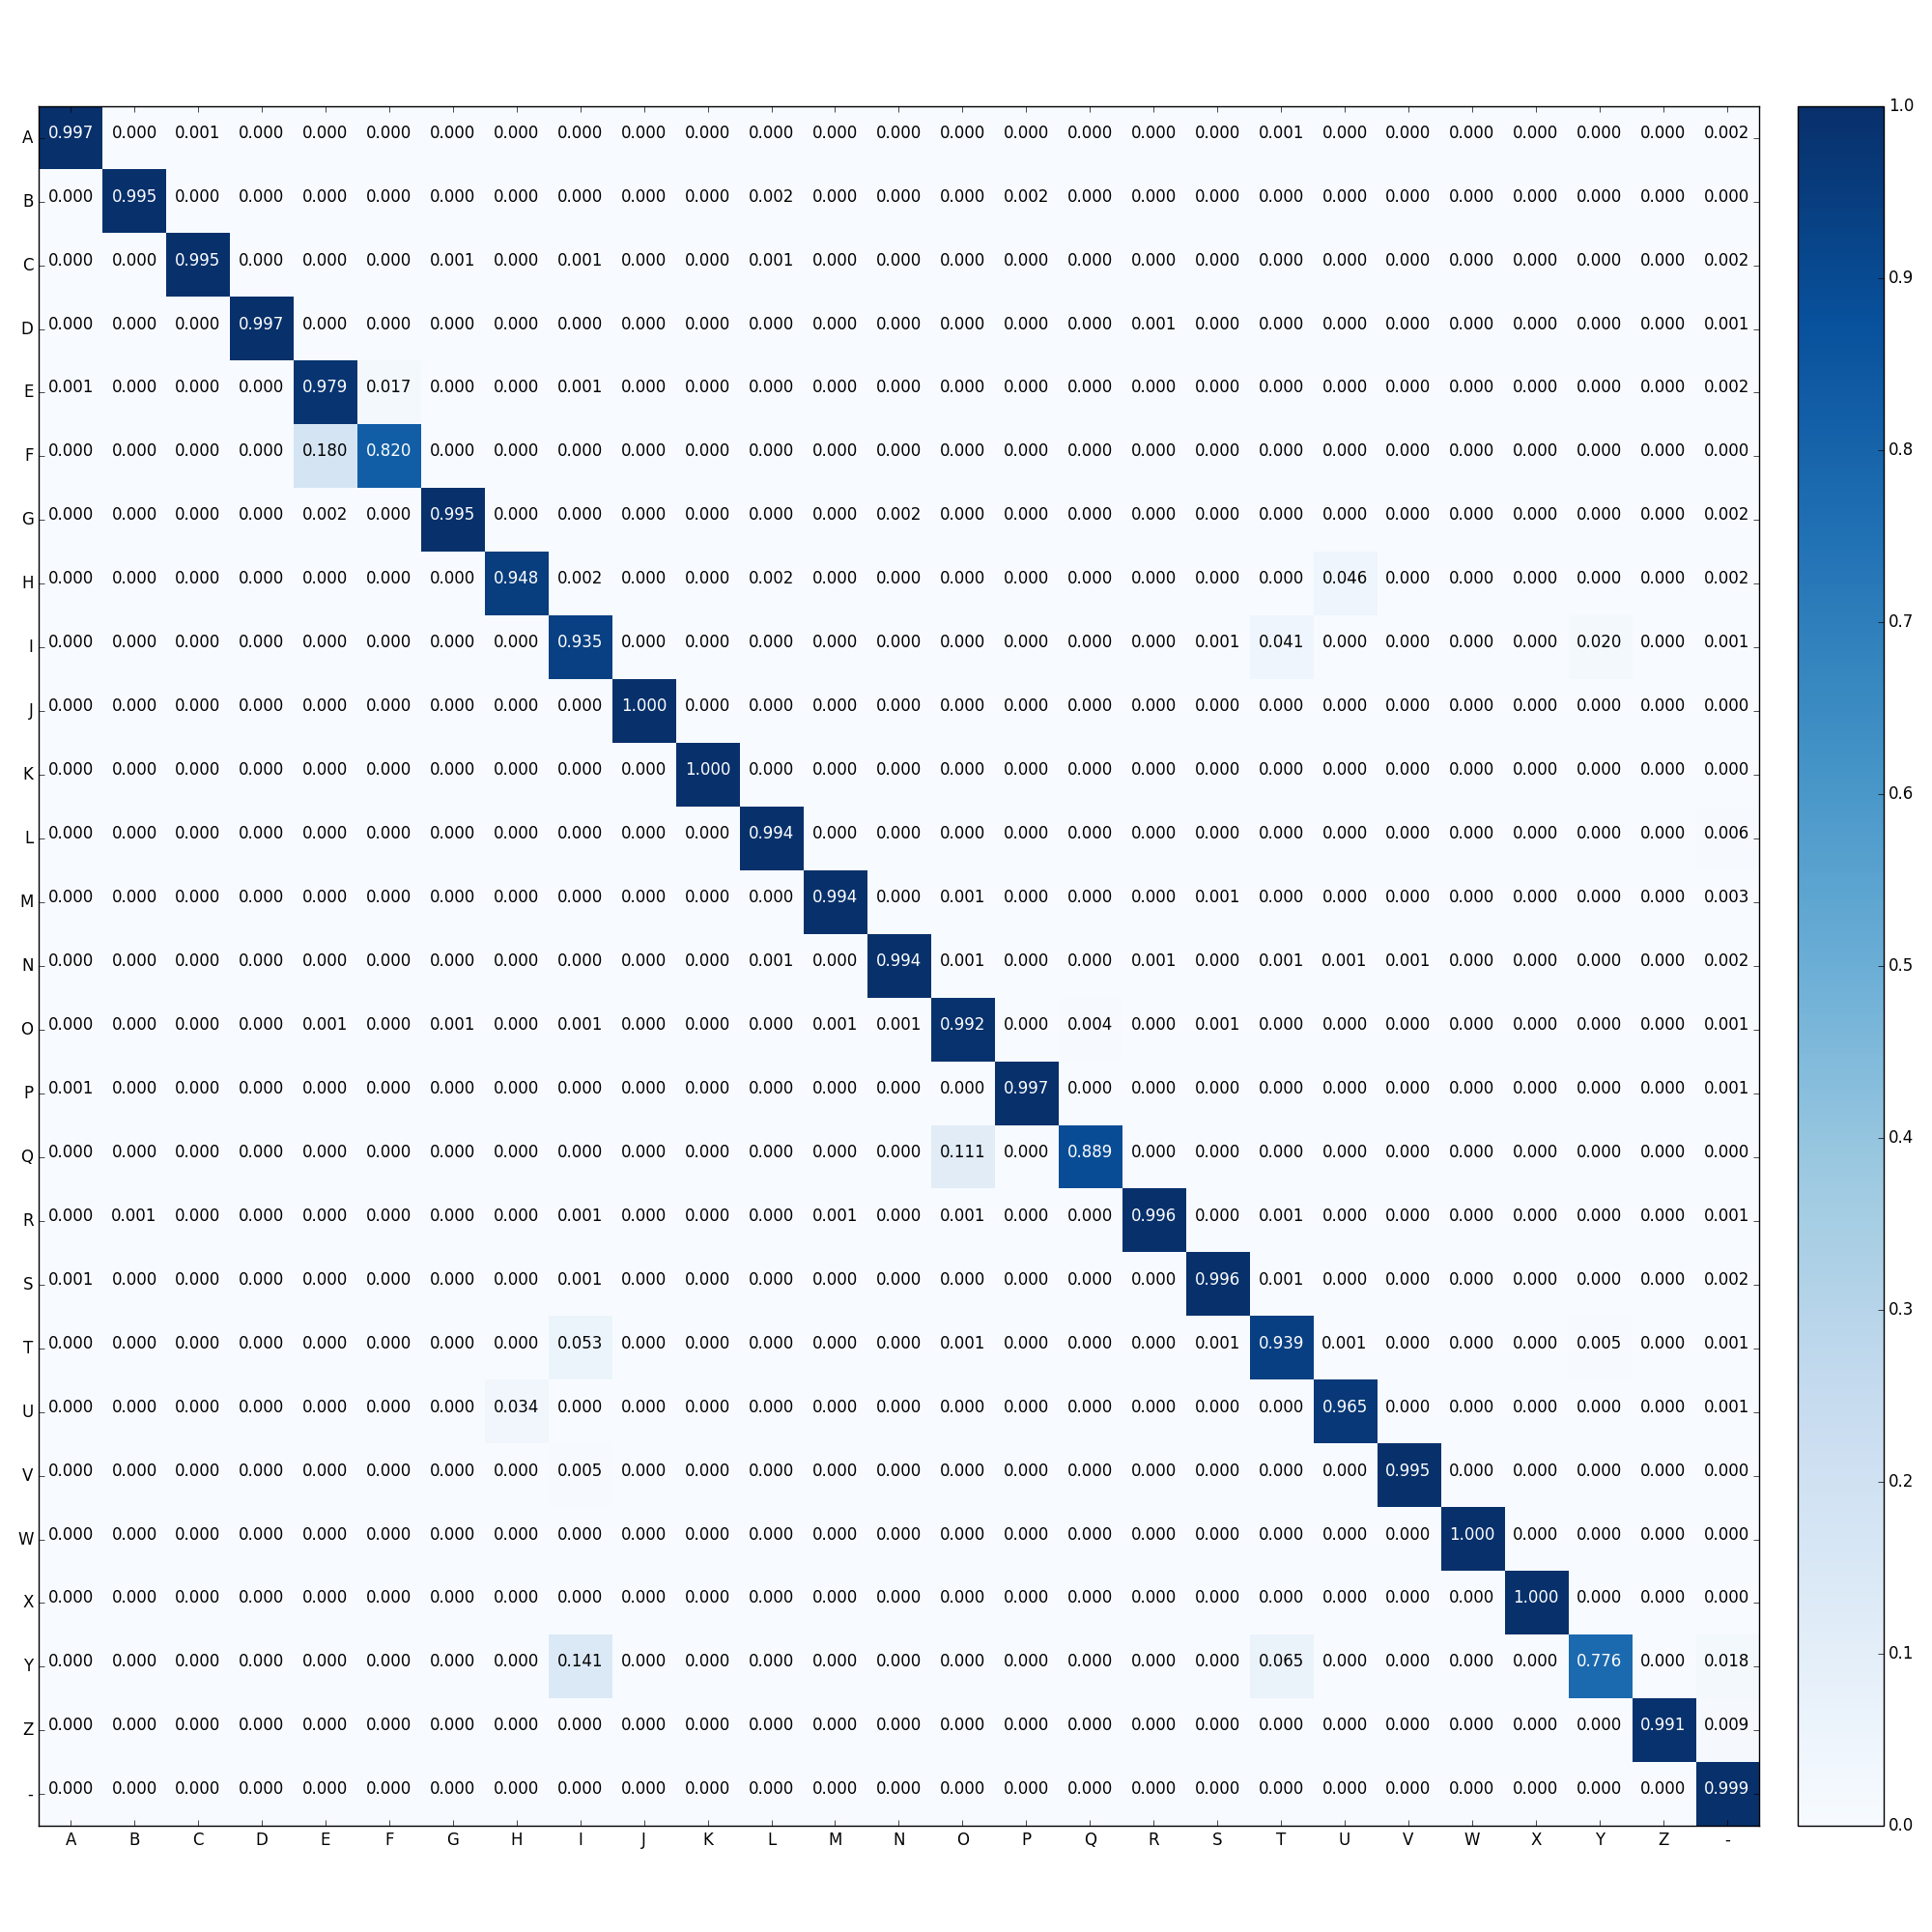
\includegraphics[width=1\textwidth]{fig/results/experiment1/big/encdecatt/confusion_matrix.png}
    \caption{Confusion matrix for the best {\tt EncDecAtt} model on the big dataset}
    \label{fig:result1_big_encdecatt_confusion_matrix}
\end{figure}

%%=========================================

\section{Handling of Two Fonts}
Table \ref{table:accuracy_two_fonts} contains the results for each model on the dataset with two fonts.

\begin{table}[H]
    \centering
    \begin{tabular}{|l|l|}
        \hline 
                                        & \textbf{Accuracy}         \\ \hline
        {\tt VecRep }                   & 40.49\%                   \\ \hline
        {\tt EncDecReg}                 & 88.21\%                   \\ \hline
        {\tt EncDecAtt}                 & \textbf{98.93\%}          \\ \hline
    \end{tabular}
    \caption{Accuracy for each model on a dataset with two fonts}
    \label{table:accuracy_two_fonts}
\end{table}

\subsection{Accuracy and Loss For Each Model}
\resultplots{fig/results/experiment2/vecrep/}{plot_accuracy_crop.png}{plot_loss_crop.png}{result2_vecrep}{Accuracy and loss for {\tt VecRep}}
\resultplots{fig/results/experiment2/encdecreg/}{plot_accuracy_crop.png}{plot_loss_crop.png}{result2_encdecreg}{Accuracy and loss for {\tt EncDecReg}}
\resultplots{fig/results/experiment2/encdecatt/}{plot_accuracy_crop.png}{plot_loss_crop.png}{result2_encdecatt}{Accuracy and loss for {\tt EncDecAtt}}

%%=========================================

\section{Noise Handling}
\red{Lorem ipsum dolor sit amet}

\begin{table}[H]
    \centering
    \begin{tabular}{|l|l|l|}
        \hline 
        \textbf{Noise factor}          & \textbf{Noise alterations}       & \textbf{Accuracy}         \\ \hline
        0\%                            & 0\%                              & 98.06\%                   \\ \hline
        5\%                            & 2.98\%                           & 93.35\%                   \\ \hline
        10\%                           & 5.46\%                           & 69.36\%                   \\ \hline
        15\%                           & 7.94\%                           & 66.77\%                   \\ \hline
        20\%                           & 10.41\%                          & 59.51\%                   \\ \hline
        40\%                           & 20.32\%                          & 47.67\%                   \\ \hline
        50\%                           & 25.28\%                          & 46.20\%                   \\ \hline
        60\%                           & 30.18\%                          & 45.29\%                   \\ \hline
    \end{tabular}
    \caption{Accuracy on the {\tt EncDecAtt} model}
    \label{table:noise_accuracy}
\end{table}

\begin{filecontents}{datax.dat}
0,0.9806
5,0.9335
10,0.6936
15,0.6677
20,0.5951
40,0.4767
50,0.4620
60,0.4529
\end{filecontents}

\begin{figure}[ht]
    \centering
    \captionsetup{justification=centering}
    \begin{tikzpicture}
        \begin{axis}[
            xmin=0, xmax=60,
            ymin=0, ymax=1,
            minor y tick num={5},
            minor x tick num={1},
            ylabel=accuracy,
            xlabel=noise,
        ]
            \addplot[draw=red] table[x index=0,y index=1,col sep=comma]{datax.dat};
        \end{axis}%
    \end{tikzpicture}%
    \caption{Change of accuracy as the amount of noise is increased}
    \label{fig:noise_accuracy}
\end{figure}

\section{Stress Test}
Att = 0.7509647 accuracy